\documentclass[
11pt, % The default document font size, options: 10pt, 11pt, 12pt
%codirector, % Uncomment to add a codirector to the title page
]{charter} 


% El títulos de la memoria, se usa en la carátula y se puede usar el cualquier lugar del documento con el comando \ttitle
\titulo{Sistema de dosificación controlada y autoajustable de líquidos aplicado a procesos industriales} 

% Nombre del posgrado, se usa en la carátula y se puede usar el cualquier lugar del documento con el comando \degreename
\posgrado{Carrera de Especialización en Sistemas Embebidos} 
%\posgrado{Carrera de Especialización en Internet de las Cosas} 
%\posgrado{Carrera de Especialización en Inteligencia Artificial}
%\posgrado{Maestría en Sistemas Embebidos} 
%\posgrado{Maestría en Internet de las cosas}
% IMPORTANTE: no omitir titulaciones ni tildación en los nombres, también se recomienda escribir los nombres completos (tal cual los tienen en su documento)
% Tu nombre, se puede usar el cualquier lugar del documento con el comando \authorname
\autor{Ing. Federico Leonardo Alderisi}

% El nombre del director y co-director, se puede usar el cualquier lugar del documento con el comando \supname y \cosupname y \pertesupname y \pertecosupname
\director{Ing. César Fabián Boarelli}
\pertenenciaDirector{UTN - FRM} 
\codirector{} % para que aparezca en la portada se debe descomentar la opción codirector en los parámetros de documentclass -> {} %Título y Nombre del codirector
\pertenenciaCoDirector{FIUBA}

% Nombre del cliente, quien va a aprobar los resultados del proyecto, se puede usar con el comando \clientename y \empclientename
\cliente{Ing. Carmelo Alderisi}
\empresaCliente{-}
 
\fechaINICIO{23 de abril de 2024}		%Fecha de inicio de la cursada de GdP \fechaInicioName
\fechaFINALPlan{11 de junio de 2024} 	%Fecha de final de cursada de GdP
\fechaFINALTrabajo{15 de mayo de 2024}	%Fecha de defensa pública del trabajo final


\begin{document}

\maketitle
\thispagestyle{empty}
\pagebreak


\thispagestyle{empty}
{\setlength{\parskip}{0pt}
\tableofcontents{}
}
\pagebreak


\section*{Registros de cambios}
\label{sec:registro}


\begin{table}[ht]
\label{tab:registro}
\centering
\begin{tabularx}{\linewidth}{@{}|c|X|c|@{}}
\hline
\rowcolor[HTML]{C0C0C0} 
Revisión & \multicolumn{1}{c|}{\cellcolor[HTML]{C0C0C0}Detalles de los cambios realizados} & Fecha      \\ \hline
0      & Creación del documento                                 &\fechaInicioName \\ \hline
1      & Se completa hasta el punto 5 inclusive                & {6} de {mayo} de 2024 \\ \hline
2      & Se completa hasta el punto 9 inclusive					& {14} de {mayo} de 2024 \\ \hline
%		  Se puede agregar algo más \newline
%		  En distintas líneas \newline
%		  Así                                                    & {día} de {mes} de 202X \\ \hline
3      & Se completa hasta el punto 12 inclusive                & {21} de {mayo} de 2024 \\ \hline
4      & Se completa el plan	                                 & {día} de {mes} de 202X \\ \hline

% Si hay más correcciones pasada la versión 4 también se deben especificar acá

\end{tabularx}
\end{table}

\pagebreak



\section*{Acta de constitución del proyecto}
\label{sec:acta}

\begin{flushright}
Buenos Aires, \fechaInicioName
\end{flushright}

\vspace{2cm}

Por medio de la presente se acuerda con el \authorname\hspace{1px} que su Trabajo Final de la \degreename\hspace{1px} se titulará ``\ttitle'' y consistirá en la implementación de un prototipo de un sistema de control de dosificación de líquidos industriales, de forma controlada y autoajustable, mediante un parámetro externo provisto por el usuario. El trabajo tendrá un presupuesto preliminar estimado de 615 horas y un costo estimado de \$4.795.200, con fecha de inicio el \fechaInicioName\hspace{1px} y fecha de presentación pública a definir.

Se adjunta a esta acta la planificación inicial.

\vfill

% Esta parte se construye sola con la información que hayan cargado en el preámbulo del documento y no debe modificarla
\begin{table}[ht]
\centering
\begin{tabular}{ccc}
\begin{tabular}[c]{@{}c@{}}Dr. Ing. Ariel Lutenberg \\ Director posgrado FIUBA\end{tabular} & \hspace{2cm} & \begin{tabular}[c]{@{}c@{}}\clientename \\ \empclientename \end{tabular} \vspace{2.5cm} \\ 
\multicolumn{3}{c}{\begin{tabular}[c]{@{}c@{}} \supname \\ Director del Trabajo Final\end{tabular}} \vspace{2.5cm} \\
\end{tabular}
\end{table}

\section{1. Descripción técnica-conceptual del proyecto a realizar}
\label{sec:descripcion}

Un dosificador de líquidos, utilizado en procesos industriales, facilita el control de las dosis aplicadas de manera controlada, continua y precisa durante un proceso específico. Generalmente, estos sistemas incorporan un medio de bombeo que permite un flujo de líquido hacia la salida del dosificador y un caudalímetro para el sensado del caudal.

Comúnmente, los sistemas de dosificación controlada constan de un único parámetro de referencia, llamado punto de trabajo. Su valor es ingresado por el usuario y representa la dosis o caudal que se desea mantener de forma continua a la salida del dosificador. El lazo cerrado del control del sistema se ajusta a través de un circuito que adquiere la señal del caudalímetro, la compara con la del punto de trabajo ingresado por el usuario y ajusta la salida para lograrlo.

A continuación, en la figura \ref{fig:diagCaudalimetroGenerico} se ilustra un sistema dosificador continuo y controlado utilizado en la industria actualmente.

\vspace{25px}
\begin{figure}[htpb]
\centering 
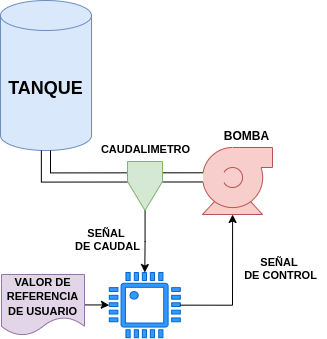
\includegraphics[width=.45\textwidth]{./Figuras/diagCaudalimetroGenerico.png}
\caption{Dosificador genérico.}
\label{fig:diagCaudalimetroGenerico}
\end{figure}


A pesar de ser un sistema utilizado en distintos procesos industriales, los sistemas de dosificación actuales no pueden transportarse ya que están fijos en una etapa del proceso. Además, estos controlan grandes o medianos caudales y su punto de trabajo se mantiene constante. En consecuencia, aquellas aplicaciones que requieran transportar un dosificador a distintos lugares o utilizar un parámetro de referencia variable para la dosificación, no pueden llevarse a cabo.

A raíz de esta problemática, se decide realizar un prototipo de un nuevo sistema de dosificación portable e innovador. A este sistema de dosificación controlada se le añade, como característica principal, la posibilidad de que el parámetro de referencia sea autoajustable, a través de un parámetro variable, en vez de uno estático como es el caso de los sistemas actuales. Además, se incorporará una interfaz de usuario que permita la interacción y configuración del sistema, como el parámetro de referencia variable, visualización de estadísticas y otras funcionalidades a definir. 

También, se utilizarán distintos subsistemas de control y alarma para el nivel del líquido del tanque, medición de temperatura y control del sistema eléctrico de alimentación. Como enfoque principal de aplicación, se desarrollará un sistema de dosificación de líquidos para aplicaciones industriales de bajo caudal.

La característica de autoajustable permite la introducción de un parámetro de referencia variable, lo que facilita el autoajuste del sistema de dosificación para adaptar el caudal de salida a las condiciones cambiantes del proceso. Esto es importante, ya que distintos procesos industriales requieren ajustes de caudal constantes. El éxito de estos procesos depende de variar el caudal en función de la magnitud de ciertos parámetros variables, como puede ser la temperatura, el peso y otros.

A continuación, en la figura \ref{fig:diagBloquesGeneral} se ilustra un diagrama en bloques del sistema propuesto. Se pueden observar los distintos bloques que conforman el sistema electrónico y el bloque del sistema eléctrico de alimentación que se desarrollará durante este trabajo. El sistema electromecánico no será incluido.

\begin{figure}[htpb]
\centering 
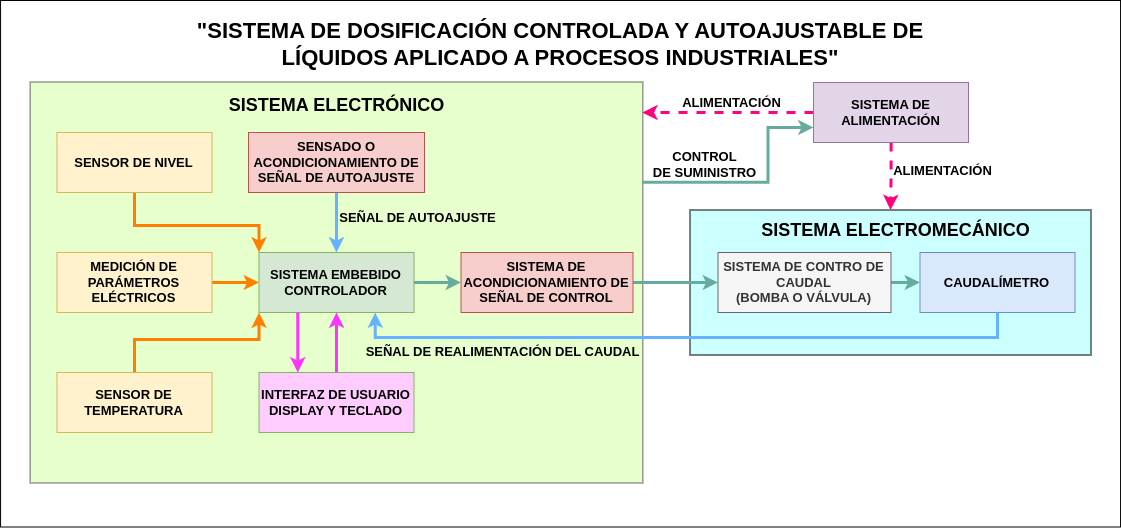
\includegraphics[width=.95\textwidth]{./Figuras/diagBloquesGeneral.png}
\caption{Diagrama en bloques del sistema.}
\label{fig:diagBloquesGeneral}
\end{figure}

Es importante destacar que este proyecto se realiza como un emprendimiento personal, junto a un colaborador que será responsable del diseño mecánico e hidráulico. Este proyecto se circunscribe al desarrollo del firmware y hardware de este sistema.

\section{2. Identificación y análisis de los interesados}
\label{sec:interesados}


\begin{table}[ht]
%\caption{Identificación de los interesados}
%\label{tab:interesados}
\begin{tabularx}{\linewidth}{@{}|l|X|X|l|@{}}
\hline
\rowcolor[HTML]{C0C0C0} 
Rol           & Nombre y Apellido & Organización 	& Puesto 	\\ \hline
%Auspiciante   &                   &              	&        	\\ \hline
Cliente       & \clientename      &\empclientename	& Consultor comercial	\\ \hline
%Impulsor      &                   &              	&        	\\ \hline
Responsable   & \authorname       & FIUBA        	& Alumno 	\\ \hline
Colaboradores & Ing. Julián Marchese                  & -              	& Diseñador       	\\ \hline
Orientador    & \supname	      & UTN - FRM 	& Director del Trabajo Final \\ \hline
%Equipo        & miembro1 \newline 
%				miembro2          &              	&        	\\ \hline
%Opositores    &                   &              	&        	\\ \hline
Usuario final & Trabajador del área industrial                   & -  & Proceso industrial   	\\ \hline
\end{tabularx}
\end{table}

Las características principales de cada uno de los interesados listados previamente son:

\begin{itemize}
	\item Cliente: ingeniero agrónomo de amplia experiencia en la industria alimentaria, agropecuaria y en el área comercial. Es una persona rigurosa y exigente al observar posibles mejoras en procesos industriales. Busca agilizar y eficientizar procedimientos y mecanismos agrícolas. La amplia experiencia permite que se pueda disponer de información respecto a los diferentes campos de aplicación del sistema a desarrollar, como así también los requerimientos mínimos a cumplir. 
	\item Colaborador: ingeniero electromecánico que trabaja como diseñador y desarrollador de sistemas mecánicos, térmicos e hidráulicos. Una persona que trabaja de forma profesional, que al desarrollar proyectos busca de forma exhaustiva cumplir con sus objetivos. Consta de un amplio conocimiento en maquinarias agropecuarias de siembra y cosecha, en los que puede ser aplicado el sistema a desarrollar.
	\item Orientador: ingeniero electrónico, domina las técnicas de diseño y armado de circuitos electrónicos de baja potencia y electrónica de baja escala de integración. Amplia experiencia en diseño asistido por computadora de sistemas de control, temperatura, presión, caudal, compensadores y PID. En la actualidad se encuentra realizando la maestría en Energía Renovables. Consta de una extensa formación complementaria en el área de sistemas control. Es un profesor comprometido con la modernización del área educacional e impulsa el perfeccionamiento de los trabajos desarrollados en el ámbito académico.
	\item Usuario final: trabajador del área industrial. Específicamente es un operario con conocimientos en la aplicación específica de su proceso industrial, que incluye dosificación de líquidos. Busca agilizar y controlar el proceso del que es responsable, utilizando una interfaz de usuario amigable y robusta. El conocimiento de las nuevas tecnologías puede variar entre distintos operarios, por lo que busca simpleza en las herramienta que utiliza.
\end{itemize}


\section{3. Propósito del proyecto}
\label{sec:proposito}

Se propone el desarrollo de un sistema prototipo de dosificación controlada y continua para líquidos en aplicaciones industriales. Este sistema permitirá autoajustarse en función de un parámetro externo dinámico o un parámetro estático ingresado por el usuario. Dado su enfoque en dosificación de bajo caudal, se diseñará para ser fácilmente transportable y con dimensiones adecuadas para ser manipulado por una persona. Este sistema constará de varios subsistemas, incluyendo una interfaz de usuario para el ingreso de parámetros de control y visualización, control de parámetros ambientales y eléctricos, así como control de nivel de tanque, entre otros.

La implementación de este sistema resuelve la problemática actual relacionada con la dificultad para mantener un flujo de dosificación autoajustable. Los sistemas de bajo costo disponibles en la actualidad no incorporan esta característica y carecen de portabilidad. Por lo tanto, el objetivo de este desarrollo es ofrecer una solución robusta, confiable y segura para su uso industrial. Esto permitirá a los usuarios reemplazar los antiguos procedimientos de dosificación aproximada en sus procesos industriales.

\section{4. Alcance del proyecto}
\label{sec:alcance}

Como se especificó en la sección \ref{sec:descripcion}, el prototipo del sistema de dosificador controlada y autoajustable consta de distintas características. Estas determinan el alcance de este trabajo final correspondiente a la  \degreename\hspace{1px}.

Este proyecto incluye:

\begin{itemize}
	\item Desarrollo del prototipo funcional del sistema de dosificación controlada y autoajustable, consta de:
			\begin{itemize}
	\item Definición del algoritmo de control para la dosificación de líquidos.
	\item Desarrollo del sistema de acondicionamiento señales de control y señales de realimentación.
	\item Implementación del algoritmo de control en un sistema embebido.
	\item Diseño e implementación de una interfaz de usuario para controlar y visualizar el funcionamiento del sistema.
	\item Adquisición de parámetros ambientales y eléctricos requeridos.
	\item Determinar un sistema de alimentación acorde al uso.
			\end{itemize}
	\item Pruebas funcionales y de concepto.
	\item Reporte de resultados.
\end{itemize}

Este proyecto no incluye:

\begin{itemize}
	\item Desarrollo del sistema hidráulico y mecánico.
	\item Construcción de un producto final comercial.
	\item Certificación del sistema a través de estándares.
\end{itemize}


\section{5. Supuestos del proyecto}
\label{sec:supuestos}

Para el desarrollo del presente proyecto se tiene a consideración los siguientes supuestos:

\begin{itemize}
	\item Interés del mercado y del cliente: actualmente, no existen sistemas de estas características que se puedan comparar con lo propuesto. En consecuencia, el cliente tiene interés en que se desarrolle este sistema.
	\item Disponibilidad de materiales: a pesar de que es complicado el proceso de importar productos electrónicos, es viable en este caso, ya que no se necesitan grandes cantidades para realizar un primer prototipo.
	\item Desarrollo del prototipo: este sistema solo será fabricado a nivel de prototipo, sin realizar iteraciones en su diseño.
	\item Presupuesto: este proyecto tendrá los fondos disponibles para financiar los gastos de inversión inicial y desarrollo.
	\item Tiempo: se dispondrá del tiempo establecido por la planificación para lograr los objetivos.
\end{itemize}


\section{6. Requerimientos}
\label{sec:requerimientos}

\begin{enumerate}
	\item Requerimientos funcionales:
		\begin{enumerate}
			\item Control:
			\begin{enumerate}
			\item El prototipo debe permitir controlar el caudal de líquido dosificado en milímetros cúbicos por minuto.
			\item La muestra de caudal debe poder ser adquirida desde una señal provista por un caudalímetro.
			\item La señal de salida del sistema de control debe permitir ser aplicada sobre un dispositivo de accionamiento, como una bomba o válvula, a definir durante el desarrollo.
			\item El sistema de control debe permitir que el usuario ingrese un valor como punto de trabajo o admitir un valor de referencia externo que funcione como punto de trabajo variable.
			\item El sistema debe permitir dosificar en forma continua, teniendo en cuenta el nivel del líquido del tanque y los límites de dosificación (entre trescientos y un valor a definir durante el transcurso del proyecto, medido en milímetros cúbicos por minuto).
			\item El sistema debe lograr el equilibrio en un tiempo acotado, en función del proceso en el que se utilizará, siendo este tiempo menor a 3 segundos.			
			\item El valor de referencia externo debe ser un valor acondicionado, que provenga de una entrada del sistema embebido utilizado.
			\item El sistema de alimentación debe ser monitoreado para mantener la integridad del dosificador.
			\item Otros parámetros a definir, como temperatura o variables del sistemas, deben poder ser monitoreados.
			\end{enumerate}
			\item Interfaz de usuario:
			\begin{enumerate}
			\item La interfaz debe permitir configurar la dosis y cambiar el modo de funcionamiento.
			\item La pantalla debe presentar el estado general del dosificador, su modo de funcionamiento, las estadísticas, configuraciones y posibles alarmas a definir.
			\item El teclado debe permitir ingresar el valor de dosificación de forma numérica, además de incluir las funciones para cambiar de menú, encender y apagar la bomba, y navegar dentro del menú.
			\item El prototipo debe mostrar señales lumínicas en función del estado de la alimentación, modo de funcionamiento y alarmas.
			\end{enumerate}
			\item Alimentación:
			\begin{enumerate}
			\item El sistema de alimentación debe poder ser conectado a una línea de alimentación de 12 Volts C.C. y adaptar esta tensión a lo requerido por el dosificador.
			\item El usuario debe poder encender o apagar el sistema de alimentación y, en consecuencia, el dosificador.
			\item El controlador debe poder apagar el sistema de alimentación, como así también limitar y aislar los puntos de falla, como el sistema de accionamiento a definir.
			\end{enumerate}
		\end{enumerate}
		
	\item Requerimientos de documentación:
		\begin{enumerate}
			\item Se debe documentar de manera clara las instrucciones de uso del dosificador.
			\item El sistema de control, junto a sus entradas y salidas, debe ser especificado eléctricamente para realizar su posterior conexión.
			\item Se debe documentar las conexiones de alimentación y del sistema electromecánico para su puesta en marcha.
		\end{enumerate}
		
	\item Requerimiento de testing y pruebas:
		\begin{enumerate}
			\item Se deben presentar resultados de las pruebas unitarias y de integración, con alcance a definir.
			\item Se deben realizar pruebas de aceptación en presencia del cliente.
			\item Las pruebas del sistema deben evidenciar los objetivos propuestos en este trabajo.
		\end{enumerate}
		
	\item Requerimientos de comunicación (opcional): el desarrollador podría proponer un sistema de comunicación inalámbrico, que permita al usuario conectarse a través de un celular, que permita configurar el sistema y visualizar datos.
\end{enumerate}

\section{7. Historias de usuarios (\textit{Product backlog})}
\label{sec:backlog}

En esta sección se describen las historias de usuarios y sus puntajes correspondientes. Los 3 aspectos que definirán los puntajes de las historias son los siguientes:

\begin{enumerate}
\item Dificultad: cantidad de trabajo a realizar.
\item Complejidad: complejidad del trabajo a realizar.
\item Incertidumbre: riesgo del trabajo a realizar.
\end{enumerate}

Se utilizará una escala de 3 puntos, donde el valor más alto implica mayor costo. A continuación, se listan los puntajes para cada item dentro de los \textit{Story points}.

\begin{enumerate}
\item Dificultad:
\begin{itemize}
	\item Baja: 1.
	\item Media: 2.
	\item Alta: 3.
\end{itemize}
\item Complejidad:
\begin{itemize}
	\item Baja: 1.
	\item Media: 2.
	\item Alta: 3.
\end{itemize}
\item Incertidumbre:
\begin{itemize}
	\item Baja: 1.
	\item Media: 2.
	\item Alta: 3.
\end{itemize}
\end{enumerate}

Historia de usuarios:

\begin{enumerate}
\item Operario: ``Como operario de la industria química, deseo un dosificador que permita cambiar la dosificación de forma automática para no tener que hacerlo manualmente."

\begin{itemize}
	\item Dificultad media (2): realizar un sistema de control automático que depende de un parámetro variable es algo que puede generar inestabilidades durante su control. A pesar de esto, si se definen los tiempos de accionamiento y límites, se puede realizar.
	\item Complejidad alta (3): requiere implementar un sistema de control digital, donde se controle y limite la variable de entrada y salida, para evitar oscilaciones. Si el parámetro de entrada oscila rápidamente, puede generar inestabilidades durante la dosificación, por lo que es algo que se debe caracterizar.
	\item Riesgo medio (2): en caso de que no pueda aplicarse un control automático en todos los casos, el sistema permite igualmente ingresar por teclado el punto de trabajo deseado. Por esto, el usuario podrá de todas maneras reemplazar el sistema manual que utiliza actualmente.
\end{itemize}

\textit{Story points}: 7.

\item Ingeniero agrónomo: ``Como ingeniero agrónomo quiero un sistema que permita ingresar un valor de dosis por teclado rápidamente y que sea visible, para agilizar la inyección de productos durante la siembra, constatar que este es el correcto y así evitar errores de dosificación."

\begin{itemize}
	\item Dificultad baja (1): realizar una interfaz de usuario a través de un teclado y una pantalla no es algo que requiera grandes esfuerzos.
	\item Complejidad media (2): este sistema debe ser robusto y confiable, por lo que la validación de datos, confirmación y ajustes de parámetros es indispensable. Además, se debe proveer una interfaz duradera, ya que será utilizada en el campo.
	\item Riesgo bajo (1): para lograr este objetivo, se debe analizar productos con interfaz de usuario que se utilizan actualmente en el campo. De esta manera se puede obtener una idea de qué tipo de interfaz rápida y confiable se puede utilizar. A pesar de esto, una mala interfaz puede generar molestia al momento de utilizar el dosificador.
\end{itemize}

\textit{Story points}: 4


\end{enumerate}


\section{8. Entregables principales del proyecto}
\label{sec:entregables}


Los entregables del proyecto son:

\begin{itemize}
	\item Un prototipo.
	\item Manual de usuario.
	\item Instrucciones de puesta en marcha, que incluye las especificaciones de las distintas conexiones eléctricas.
	\item Diagrama de circuitos esquemáticos.
	\item Memoria del trabajo final.
\end{itemize}


\section{9. Desglose del trabajo en tareas}
\label{sec:wbs}

A continuación, se desglosa el trabajo en tareas con su duración estimada:

\begin{enumerate}
\item Desarrollo del prototipo (395 h).

	\begin{enumerate}
	\item Modularización del sistema y definición de funcionalidades (80 h).
	
		\begin{enumerate}
		\item Selección del dispositivo de accionamiento, medición de caudal y caracterización de las señales correspondientes (20 h).
		\item Definición del sistema de control y algoritmo (30 h).
		\item Determinación de los periféricos de entrada y salida (15 h).
		\item Definición de circuitos e interfaces de acondicionamiento de señales (15 h).
		\end{enumerate}
		
	\item Selección del sistema embebido, circuitos periféricos e implementación del programa (160 h).
	
		\begin{enumerate}
		\item Selección del sistema embebido, acorde a los requerimientos y el análisis previo (15 h).
		\item Programación del sistema de control principal (40 h).
		\item Programación de drivers (40 h).
		\item Programación de la interfaz de usuario (35 h).
		\item Programación de sistemas secundarios (30 h).
		\end{enumerate}

		
	\item Hardware, sistema de alimentación, circuitos periféricos e interfaces de conexión (155 h).
	
		\begin{enumerate}
		\item Definición de dispositivos y periféricos generales (interfaz de usuario, adaptadores de señales y otros) (30 h).
		\item Diseño del sistema de alimentación (15 h).
		\item Dimensionamiento de componentes (15 h).
		\item Diseño de esquemáticos (35 h).
		\item Diseño de placas y conexionado (30 h).
		\item Ensamblaje del prototipo (20 h).
		\item Pruebas eléctricas e inspección general (10 h).
		\end{enumerate}		
		
	\end{enumerate}		
		
\item Testing (95 h).
	
	\begin{enumerate}
	\item Realizar pruebas unitarias (40 h).
	\item Realizar pruebas de integración (35 h).
	\item Realizar pruebas del sistema (20 h).
	\end{enumerate}		
		
		
\item Documentación (125 h).

	\begin{enumerate}
	\item Desarrollo de reporte de testing (25 h).
	\item Elaboración del manual e instrucciones (20 h).
	\item Redacción del informe de avance (20 h).
	\item Redacción de la memoria del trabajo final (40 h).
	\item Elaboración de la presentación del proyecto (20 h).
	\end{enumerate}

\end{enumerate}

Total de horas estimadas: 615 h.

\section{10. Diagrama de Activity On Node}
\label{sec:AoN}


En las figuras \ref{fig:actOnNode1} y \ref{fig:actOnNode2} se muestra el diagrama de Activity on Node del presente proyecto, basado en el desglose de tareas. Las referencias temporales son presentadas en horas. Las flechas en rojo muestran el camino crítico, que suma un total de 340 h.



\begin{landscape}
\begin{figure}[htpb]
\vspace{55px}
\centering 
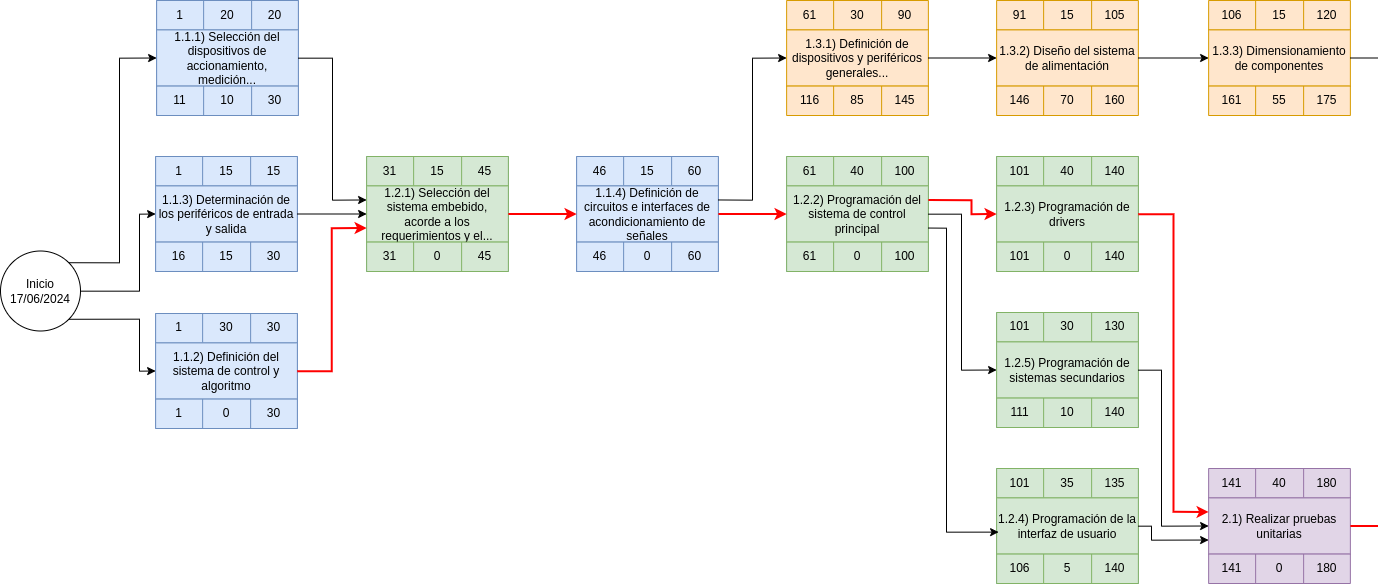
\includegraphics[height=.6\textheight]{./Figuras/actOnNode1.png}
\caption{Diagrama de \textit{Activity on Node(1).}}
\label{fig:actOnNode1}
\end{figure}
\end{landscape}

\begin{landscape}
\begin{figure}[htpb]
\vspace{55px}
\centering 
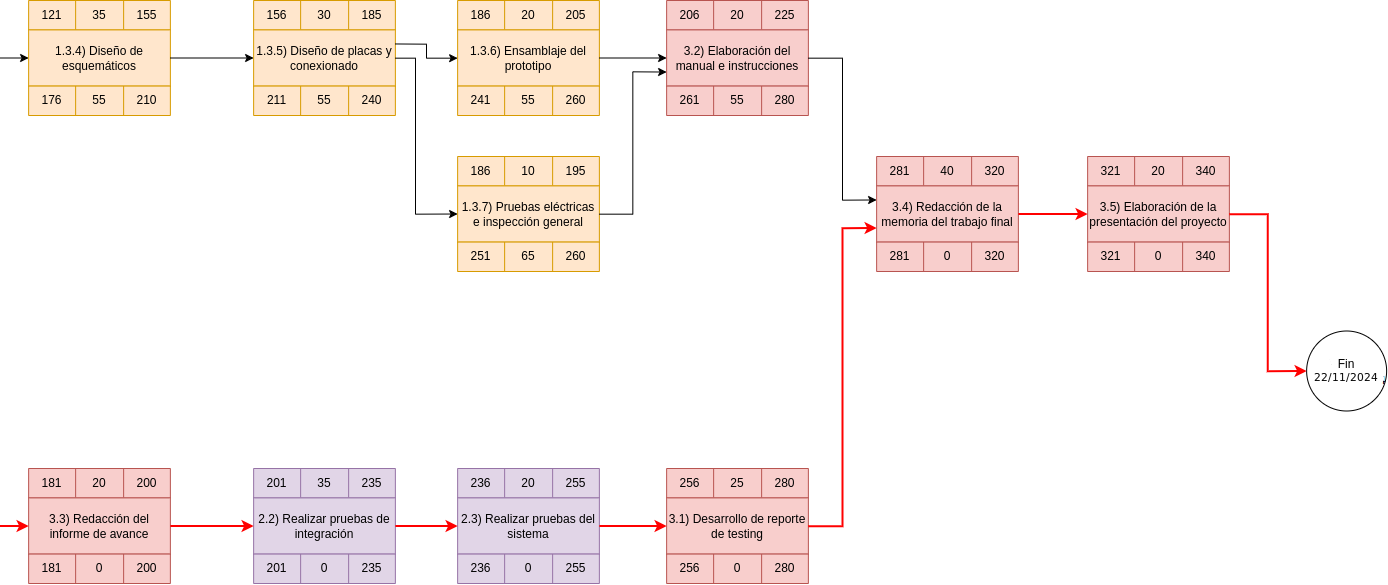
\includegraphics[height=.6\textheight]{./Figuras/actOnNode2.png}
\caption{Diagrama de \textit{Activity on Node(2).}}
\label{fig:actOnNode2}
\end{figure}
\end{landscape}


\section{11. Diagrama de Gantt}
\label{sec:gantt}

A continuación, en la figura \ref{fig:ganntTable} se muestra la tabla con la información correspondiente al desglose de tareas. Además, se observa su duración, fecha de inicio y fecha de fin. El diagrama de Gannt se puede observar en la imagen \ref{fig:ganntImag}.



\begin{figure}[htpb]
\vspace{55px}
\centering 
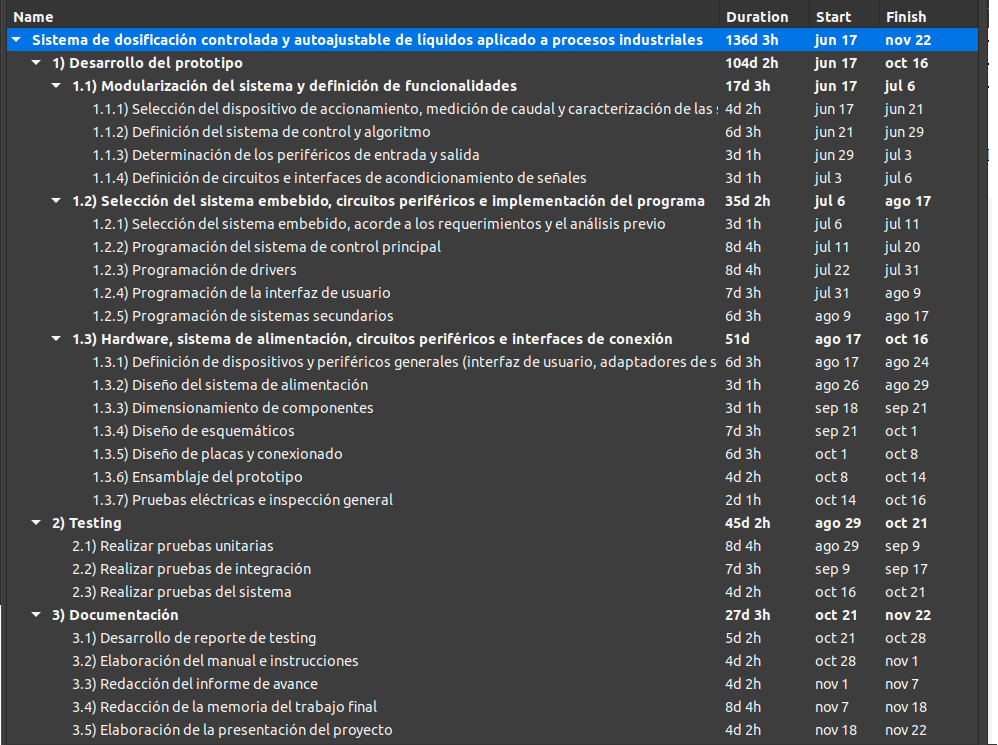
\includegraphics[height=.5\textheight]{./Figuras/ganntTable.png}
\caption{Tabla del diagrama de \textit{Gannt.}}
\label{fig:ganntTable}
\end{figure}

\begin{landscape}
\begin{figure}[htpb]
\centering 
\vspace{80px}
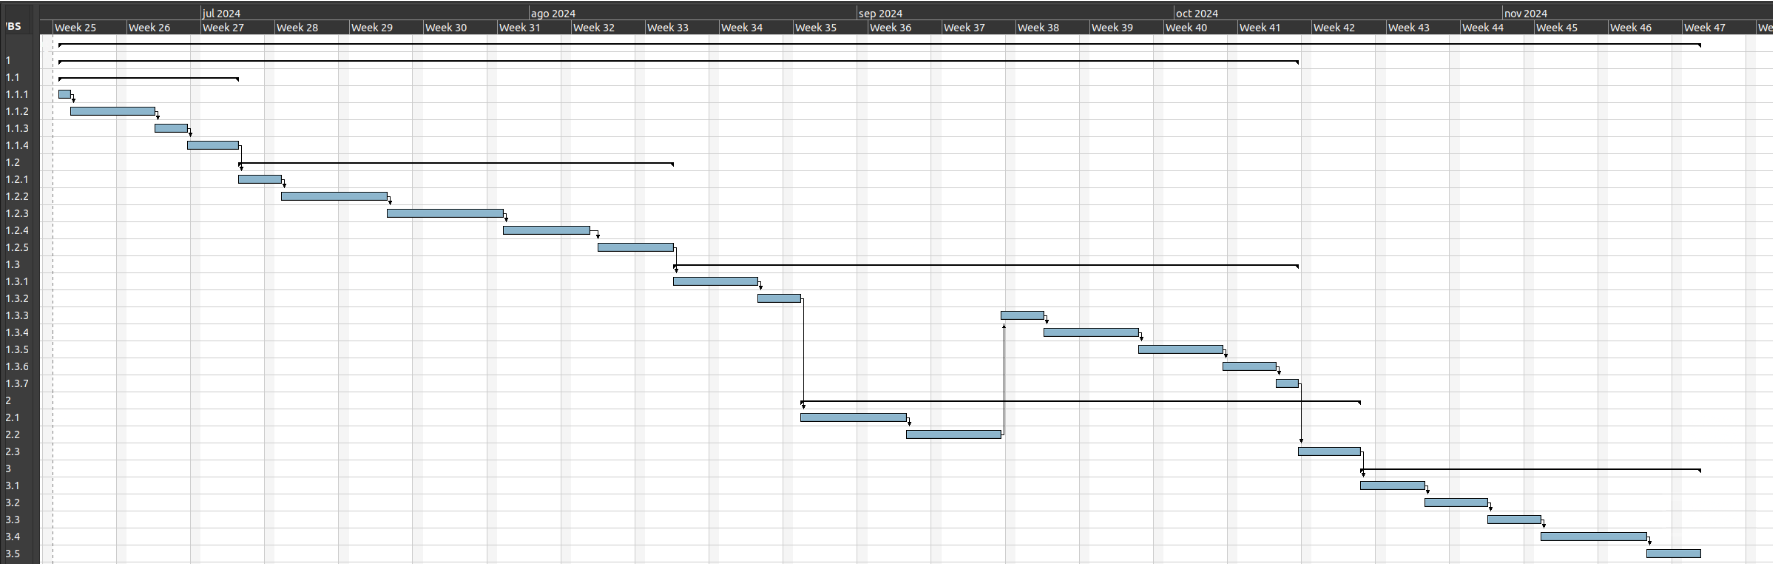
\includegraphics[height=.5\textheight]{./Figuras/ganntImag.png}
\caption{Diagrama de \textit{Gannt.}}
\label{fig:ganntImag}
\end{figure}
\end{landscape}


\section{12. Presupuesto detallado del proyecto}
\label{sec:presupuesto}

A continuación, se describen los costos aproximados del proyecto expresados en pesos argentinos. Estos costos se basan en los valores promedios que se encontraron para distintos elementos candidatos a ser utilizados, por lo que estos valores pueden verse ajustados durante el desarrollo del proyecto. El valor de 1 USD (dólar estadounidense), al momento de realizar el presupuesto, es de \$1.200.


\begin{table}[htpb]
\centering
\begin{tabularx}{\linewidth}{@{}|X|c|r|r|@{}}
\hline
\rowcolor[HTML]{C0C0C0} 
\multicolumn{4}{|c|}{\cellcolor[HTML]{C0C0C0}COSTOS DIRECTOS} \\ \hline
\rowcolor[HTML]{C0C0C0} 
Descripción &
  \multicolumn{1}{c|}{\cellcolor[HTML]{C0C0C0}Cantidad} &
  \multicolumn{1}{c|}{\cellcolor[HTML]{C0C0C0}Valor unitario} &
  \multicolumn{1}{c|}{\cellcolor[HTML]{C0C0C0}Valor total} \\ \hline
  
  \multicolumn{1}{|l|}{Horas de ingeniería}&
  \multicolumn{1}{c|}{615} &
  \multicolumn{1}{c|}{\$ 5000} &
  \multicolumn{1}{c|}{\$3 250 000} \\ \hline
  
  \multicolumn{1}{|l|}{Microcontrolador}&
  \multicolumn{1}{c|}{2} &
  \multicolumn{1}{c|}{\$45 000} &
  \multicolumn{1}{c|}{\$90 000} \\ \hline
  
  \multicolumn{1}{|l|}{Manufactura de PCB}&
  \multicolumn{1}{c|}{5} &
  \multicolumn{1}{c|}{\$10 000} &
  \multicolumn{1}{c|}{\$50 000} \\ \hline
  
  \multicolumn{1}{|l|}{Componentes pasivos}&
  \multicolumn{1}{c|}{300} &
  \multicolumn{1}{c|}{\$100} &
  \multicolumn{1}{c|}{\$30 000} \\ \hline
  
  \multicolumn{1}{|l|}{Fuente de alimentación}&
  \multicolumn{1}{c|}{2} &
  \multicolumn{1}{c|}{\$3500} &
  \multicolumn{1}{c|}{\$7000} \\ \hline

  \multicolumn{1}{|l|}{Conectores, borneras y otros}&
  \multicolumn{1}{c|}{5} &
  \multicolumn{1}{c|}{\$10 000} &
  \multicolumn{1}{c|}{\$50 000} \\ \hline
  
  \multicolumn{1}{|l|}{Sensores}&
  \multicolumn{1}{c|}{2} &
  \multicolumn{1}{c|}{\$17 500} &
  \multicolumn{1}{c|}{\$35 000} \\ \hline
  
  \multicolumn{1}{|l|}{Caja estanca}&
  \multicolumn{1}{c|}{1} &
  \multicolumn{1}{c|}{\$15 000} &
  \multicolumn{1}{c|}{\$15 000} \\ \hline
  
  \multicolumn{1}{|l|}{Interfaz gráfica y teclado}&
  \multicolumn{1}{c|}{1} &
  \multicolumn{1}{c|}{\$25 000} &
  \multicolumn{1}{c|}{\$25 000} \\ \hline

\multicolumn{3}{|c|}{SUBTOTAL} &
  \multicolumn{1}{c|}{\$3 552 000} \\ \hline
  
\rowcolor[HTML]{C0C0C0} 
\multicolumn{4}{|c|}{\cellcolor[HTML]{C0C0C0}COSTOS INDIRECTOS} \\ \hline
\rowcolor[HTML]{C0C0C0} 
Descripción &
  \multicolumn{1}{c|}{\cellcolor[HTML]{C0C0C0}Cantidad} &
  \multicolumn{1}{c|}{\cellcolor[HTML]{C0C0C0}Valor unitario} &
  \multicolumn{1}{c|}{\cellcolor[HTML]{C0C0C0}Valor total} \\ \hline
  
  \multicolumn{1}{|l|}{35\% de los costos directos}&
  \multicolumn{1}{c|}{1} &
  \multicolumn{1}{c|}{\$1 243 200} &
  \multicolumn{1}{c|}{\$1 243 200} \\ \hline
  
\multicolumn{3}{|c|}{SUBTOTAL} &
  \multicolumn{1}{c|}{\$1 243 200} \\ \hline
\rowcolor[HTML]{C0C0C0}
\multicolumn{3}{|c|}{TOTAL} &
\multicolumn{1}{c|}{\$4 795 200} \\ \hline

\end{tabularx}
\end{table}


\section{13. Gestión de riesgos}
\label{sec:riesgos}


a) En la siguiente sección se describen los principales riesgos, sus consecuencias y se estima la importancia a partir del análisis de los siguientes parámetros:

\begin{enumerate}
\item Severidad (S): se evalúa del 1 al 10, siendo el 10 el grado más alto de importancia y consecuencias.
\item Probabilidad de ocurrencia (O): se evalúa del 1 al 10, siendo el 10 el grado más alto de probabilidad de ocurrencia.
\item Nivel de prioridad de riesgo (RPN): se obtiene al realizar el producto de la \textit{Severidad (S)} y la \textit{Probabildad de ocurrencia (O)}, este representa un nivel relativo y comparativo del nivel de importancia.
\end{enumerate}

Riesgo 1: demora de entrega al importar dispositivos o faltante de estos.
\begin{itemize}
	\item Severidad (S): 8, esto impacta fuertemente ya que el desarrollo y las pruebas dependen de los dispositivos y controladores.
	\item Ocurrencia (O): 7, esto suele suceder frecuentemente, a mediad que el precio de la encomienda es mayor.
\end{itemize}

Riesgo 2: dificultad durante el desarrollo del sistema de control.
\begin{itemize}
	\item Severidad (S): 7, esto genera una complicación importante ya que el principal objetivo del proyecto es el desarrollo e implementación de un sistema de control.
	\item Ocurrencia (O): 4, el sistema de control a implementar no requiere un desarrollo completamente desconocido. Existen implementaciones y casos similares de aplicación, en donde se puede recopilar información afín.
\end{itemize}

Riesgo 3: destrucción del prototipo durante las pruebas.
\begin{itemize}
	\item Severidad (S): 9, la destrucción del prototipo implica la perdida del entregable principal.
	\item Ocurrencia (O): 7, esto es posible ya que las pruebas funcionales requieren ser realizadas en el campo de aplicación, junto a los equipos electromecánicos.
\end{itemize}

Riesgo 4: elevados costos de componentes y materiales.
\begin{itemize}
	\item Severidad (S): 4, ya que este proyecto no requiere componentes que impliquen gran inversión, a pesar de que puedan tener un aumento a corto plazo.
	\item Ocurrencia (O): 5, es probable que aumenten los precios de los dispositivos electrónicos durante un posible conflicto bélico en los países asiáticos donde se realiza la manufactura (como China y Taiwan).
\end{itemize}

Riesgo 5: modificación del alcance del proyecto durante el desarrollo.
\begin{itemize}
	\item Severidad (S): 7, esto modifica notablemente la planificación, el tiempo y el costo del desarrollo.
	\item Ocurrencia (O): 3, esto tiene baja ocurrencia ya que se realizó un estudio previo amplio a través de encuestas a posibles usuarios.
\end{itemize}

b) En la siguiente tabla de gestión de riesgos se representan los niveles de prioridad para los riesgos listados anteriormente:

Criterio adoptado: se tomarán medidas de mitigación en los riesgos cuyos números de RPN sean mayores a 40. 

\begin{table}[htpb]
\centering
\begin{tabularx}{\linewidth}{@{}|X|c|c|c|c|c|c|@{}}
\hline
\rowcolor[HTML]{C0C0C0} 
Riesgo & S & O & RPN & S* & O* & RPN* \\ \hline
   Riesgo 1: demora de entrega al importar dispositivos o faltante de estos.    & 8  & 7  &  56   &  8  &  3  &  24    \\ \hline
   Riesgo 2: dificultad durante el desarrollo del sistema de control.    & 7  & 4  &  28   &  -  &  -  &   -   \\ \hline
   Riesgo 3: destrucción del prototipo durante las pruebas.    & 9  & 7  &  63   &  4  & 7   &  28    \\ \hline
   Riesgo 4: elevados costos de componentes y materiales.    &  4 & 5  &  20   &  -  &  -  &   -   \\ \hline
   Riesgo 5: modificación del alcance del proyecto durante el desarrollo.    & 7  & 3  &  21   &  -  &  -  &   -   \\ \hline
\end{tabularx}%
\end{table}

c) Plan de mitigación de los riesgos que originalmente excedían el RPN máximo establecido:

Riesgo 1: se definirán los dispositivos a utilizar con anticipación, para acortar los posibles retrasos. Además, se buscarán distintos proveedores internos y externos, priorizando los internos, para evitar las complicaciones que se generan durante la importación. EN caso de importar, se intentarán realizar pequeñas compras para evitar detención de la encomienda en la aduana.

  \begin{itemize}
	\item Severidad (S*): 8, si sucede. impacta igualmente en el desarrollo.
	\item Probabilidad de ocurrencia (O*): 3, ya que al priorizar los proveedores internos, se disminuye la probabilidad de los problemas al importar pequeñas cantidades de dispositivos.
	\end{itemize}

Riesgo 3: está previsto realizar un prototipo de respaldo, para que en caso de falla o destrucción, aún exista la posibilidad de proveer el entregable principal. Este tendrá las mismas características funcionales que el prototipo principal.
  \begin{itemize}
	\item Severidad (S*): 4, a pesar de que existe un prototipo de respaldo, este no será el original con el que se realizarán todas las pruebas, sino es solo un respaldo.
	\item Probabilidad de ocurrencia (O*): 7, la probabilidad no disminuye ya que las pruebas se deben realizar igualmente y el riesgo de fallas se mantiene.
	\end{itemize}


\section{14. Gestión de la calidad}
\label{sec:calidad}

En esta sección se describen las verificaciones y validaciones para los requerimientos definidos como críticos:

\begin{itemize} 
\item Req 1.1.1.1) El prototipo debe permitir controlar el caudal de líquido dosificado en milímetros cúbicos por minuto.

\begin{itemize}
	\item Verificación: se ingresarán distintos valores a través de la interfaz gráfica y se controlará el volumen del líquido expedido por el sistema luego de un minuto.
	\item Validación: el cliente inspeccionará el caudal y el volumen expedido a través un método elegido por él.
\end{itemize}

\item Req 1.1.1.2) La muestra de caudal debe poder ser adquirida desde una señal provista por un caudalímetro.

\begin{itemize}
	\item Verificación: se utilizarán distintas valores y puntos de trabajos simulando la señal de un caudalímetro real.
	\item Validación: se instalará el prototipo junto al sistema electromecánico y se conectará a la señal del caudalímetro.
\end{itemize}

\item Req 1.1.1.4) El sistema de control debe permitir que el usuario ingrese un valor como punto de trabajo o admitir un valor de referencia externo que funcione como punto de trabajo variable.

\begin{itemize}
	\item Verificación: se cambiará la configuración del parámetro de entrada del sistema de control durante su funcionamiento.
	\item Validación: se inyectará una señal que simule un parámetro variable que cambia el punto de trabajo del dosificador, observando el comportamiento a la salida del sistema.
\end{itemize}

\item Req 1.1.1.6) El sistema debe lograr el equilibrio en un tiempo acotado, en función del proceso en el que se utilizará, siendo este tiempo menor a 3 segundos.

\begin{itemize}
	\item Verificación: se calculará el tiempo de establecimiento del sistema de control.
	\item Validación: se realizarán pruebas con parámetros estáticos y variables para corroborar el tiempo de establecimiento del caudal.
\end{itemize}

\item Req 1.1.2.1) La interfaz debe permitir configurar la dosis y cambiar el modo de funcionamiento.

\begin{itemize}
	\item Verificación: se implementarán pruebas de interfaz gráfica y teclado, para verificar las distintas combinaciones de manipulación del menú y la configuración.
	\item Validación: el usuario navegará por todo los menús y configuraciones antes y durante el funcionamiento.
\end{itemize}

\item Req 1.1.2.3) El teclado debe permitir ingresar el valor de dosificación de forma numérica, además de incluir las funciones para cambiar de menú, encender y apagar la bomba, y navegar dentro del menú.

\begin{itemize}
	\item Verificación: se le entregará al cliente un documento previo con las distintas presentaciones de datos, modos de configuración y menús que tendrá el sistema.
	\item Validación: el cliente podrá corroborar lo solicitado durante la navegación en el menú del sistema.
\end{itemize}

\item Req 1.1.2.4) El prototipo debe mostrar señales lumínicas en función del estado de la alimentación, modo de funcionamiento y alarmas.

\begin{itemize}
	\item Verificación: se generarán fallas y estados de alerta que permitan corroborar las salidas del sistema de control.
	\item Validación: durante las pruebas finales, se generarán fallas para corroborar su correcto funcionamiento.
\end{itemize}

\item Req 1.1.3.1): El sistema de alimentación debe poder ser conectado a una línea de alimentación de 12 Volts C.C. y adaptar esta tensión a lo requerido por el dosificador.

\begin{itemize}
	\item Verificación: se constatarán los valores de tensión de entrada y salida del sistema de alimentación.
	\item Validación: una vez instalado el prototipo, se constatarán los valores de entrada y salida del sistema de alimentación.
\end{itemize}

\item Req 1.1.3.2): El usuario debe poder encender o apagar el sistema de alimentación y, en consecuencia, el dosificador.

\begin{itemize}
	\item Verificación: se simulará el sistema de encendido y apagado de alimentación.
	\item Validación: el cliente realizará pruebas de corte y encendido de alimentación.
\end{itemize}

\item Req 1.1.3.3): El controlador debe poder apagar el sistema de alimentación, como así también limitar y aislar los puntos de falla, como el sistema de accionamiento a definir.

\begin{itemize}
	\item Verificación: se realizarán pruebas no destructivas que simulen un estado de falla eléctrico para forzar el sistema de apagado automático.
	\item Validación: se forzará una falla de baja tensión de entrada, para generar una alarma.
\end{itemize}

\end{itemize}


\section{15. Procesos de cierre}    
\label{sec:cierre}

\begin{itemize}
	\item Pautas de trabajo que se seguirán para analizar si se respetó el Plan de Proyecto original:
		\begin{enumerate}
		\item Responsable: Federico Leonardo Alderisi.
		\item Se verificará que los requerimientos se hayan cumplido, que las verificaciones y validaciones hayan sido correctamente elegidas y si el tiempo dedicado coincidió con la planificación.
		\end{enumerate}		 
	\item Identificación de las técnicas y procedimientos útiles e inútiles que se emplearon, los problemas que surgieron y cómo se solucionaron:
		\begin{enumerate}
		\item Responsable: Federico Leonardo Alderisi.
		\item Se revisará el enfoque y métodos de programación utilizados, la elección del sistema de control y la versatilidad de la interfaz gráfica desarrollada para evaluar y listar las mejoras que podrían realizarse en futuros trabajos.
		\end{enumerate}	
	\item Indicar quién organizará el acto de agradecimiento a todos los interesados, y en especial al equipo de trabajo y colaboradores:
		\begin{enumerate}
		\item Responsable: Federico Leonardo Alderisi.
		\item Se agradecerá formalmente a los colaboradores, profesores y autoridades de la especialización, como así también al cliente y a los participantes indirectos que hicieron posible el desarrollo trabajo final.
		\end{enumerate}	
\end{itemize}	  
	  
\end{document}
